An essential step for obtaining computational proofs of geometric results is \emph{discretization}: problems concerning the existence of an object $\mathcal{O}$ in a continuous space such as $\mathbb{R}^2$ must be reformulated in terms of the existence of a discrete and finitely representable object $\mathcal{O}'$ that a computer can find (or discard its existence). 
This poses a particular challenge for problems in which the desired geometric object $\mathcal{O}$ is characterized by very specific coordinates of points, requiring to deal with floating point arithmetic or numerical stability.  
Fortunately, this is not the case for Erd\H{o}s-Szekeres-type problems such as determining the value of $h(k)$, which are naturally well-suited for computation. 
This is so because the properties of interest (e.g., convexity, emptiness) can be described in terms of high-level relationships between points and lines (e.g., point $p$ is above the line $\vec{qr}$, lines $\vec{qr}$ and $\vec{st}$ intersect, etc.), which are invariant under rotations, translations, and even small perturbations of the coordinates. This suggests the problems can be discretized in terms of boolean variables representing these high-level relationships, forgetting the specific coordinates of the points.  
The combinatorial abstraction that has been most widely used in Erd\H{o}s-Szekeres-type problems is that of \emph{triple orientations}~\cite{ emptyHexagonNumber, scheucherTwoDisjoint5holes2020}.\footnote{Also known as \emph{signotopes}~\cite{felsnerSweepsArrangementsSignotopes2001, subercaseaux2023minimizing},  Knuth's \emph{counterclockwise} relation~\cite{knuthAxiomsHulls1992}, or \emph{signatures}~\cite{szekeres_peters_2006}.}
Given points $p, q, r$, their \emph{triple-orientation} is defined as 
\newcommand{\sign}{\operatorname{sign}}
\[
  \sigma(p, q, r) = \sign \det \begin{pmatrix} p_x & q_x & r_x \\ p_y & q_y & r_y \\ 1 & 1 & 1 \end{pmatrix} = \begin{cases}
    1 & \text{if } p, q, r \text{ are \emph{oriented} counterclockwise}, \\
    0 & \text{if } p, q, r \text{ are collinear}, \\
    -1 & \text{if } p, q, r \text{ are \emph{oriented} clockwise}.
  \end{cases}.
\]

\begin{figure}
  \centering
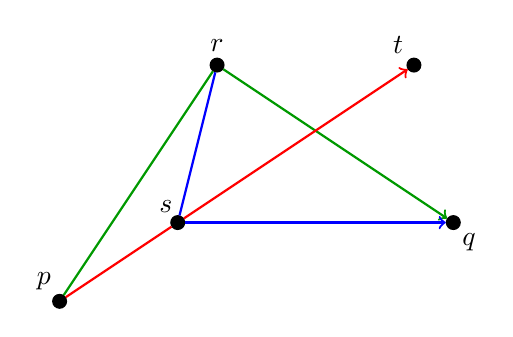
\begin{tikzpicture}
  %\draw[ultra thick, dashed, blue] (5,1) -- (0,0);
  \node[draw, circle, black, fill=black, inner sep=0pt, minimum size=5pt] (p) at (0,0) {};
  \node[] at (-0.2, 0.25) {$p$};
  \node[draw, circle, black, fill=black, inner sep=0pt, minimum size=5pt] (q) at (5,1) {};
  \node[] at (5.2, 0.75) {$q$};
  \node[draw, circle, black, fill=black, inner sep=0pt, minimum size=5pt] (r) at (2,3) {};
  \node[] at (2, 3.25) {$r$};

  \node[draw, circle, black, fill=black, inner sep=0pt, minimum size=5pt] (s) at (1.5, 1) {};
  \node[] at (1.35, 1.2) {$s$};

  \node[draw, circle, black, fill=black, inner sep=0pt, minimum size=5pt] (t) at (4.5, 3) {};
  \node[] at (4.3, 3.25) {$t$};

  \draw[ thick,  green!60!black] (p) -- (r);
  \draw[ thick,  green!60!black, ->] (r) -- (q);

  \draw[ thick,  blue] (r) -- (s);
  \draw[ thick,  blue, ->] (s) -- (q);

  \draw[thick,  red] (p) -- (s);
  \draw[thick,  red, ->] (s) -- (t);
  % \draw[fill=green, opacity=0.5] (a.center) -- (b.center) -- (c.center) -- cycle;
\end{tikzpicture}
\caption{Illustration of triple orientations, where $\sigma(p, r, q) = -1, \sigma(r, s, q) = 1, $ and $\sigma(p, s, t) = 0$.}\label{fig:triple-orientation} 
\end{figure}

An example is illustrated in~\Cref{fig:triple-orientation}. Formally, we identify points with members of $\mathbb{R}^2$, and use \textsf{mathlib}'s definition of the determinant to define $\sigma$.
% @[pp_dot] abbrev x (p : Point) : ℝ := p 0
% @[pp_dot] abbrev y (p : Point) : ℝ := p 1
\begin{lstlisting}
abbrev Point := EuclideanSpace ℝ (Fin 2)

inductive Orientation : Type
  | CW -- clockwise :=  -
  | CCW -- counter clockwise:= +
  | Collinear -- := 0

noncomputable def σ (p q r : Point) : Orientation := 
  let det := Matrix.det !![p.x, q.x, r.x ; p.y, q.y, r.y ; 1, 1, 1]
  if 0 < det then CCW
  else if det < 0 then CW
  else Collinear
\end{lstlisting}

% def Orientation.ofReal (r : ℝ) : Orientation :=
%   if 0 < r then CCW
%   else if r < 0 then CW
%   else Collinear

Through the $\sigma$ function we can immediately define the notion of \emph{general position} for collections (e.g., finite sets, lists, etc.) of points, simply establishing that $\sigma(p, q, r) \neq 0$ for every three distinct points $p, q, r$ in the collection.
Furthermore, we can start formalizing sets of points that are \emph{equivalent} with respect to their triple orientations, and consequently, properties of pointsets that are fully captured by their triple orientations~(\emph{orientation properties}).

% \begin{definition}[$\sigma$-equivalence]
%   Given two lists of points $S$ and $T$, we say that $S$ and $T$ are \emph{equivalent} with respect to their triple orientations, denoted $S \equiv_\sigma T$, if there exists a bijection $f : S \to T$ such that $\sigma(p, q, r) = \sigma(f(p), f(q), f(r))$ for every $p \neq q \neq r \in S$.
% \end{definition}

% \begin{definition}[Orientation property]
%   A property $P$ that maps lists of points to $\{\texttt{true}, \texttt{false}\}$ is an \emph{orientation property} if for every pair of lists of points $S$ and $T$ that are equivalent with respect to their triple orientations, $P(S) = P(T)$.
% \end{definition}

\begin{lstlisting}
  structure σEquiv (S T : List Point) :=
    (f : Point → Point) (permutation : S.map f ~ T)
    (σ : ∀ p q r, p ∈ S → q ∈ S → r ∈ S → σ (f p) (f q) (f r) = σ p q r)

  def OrientationProperty (P : List Point → Prop) :=
    ∀ {{S T}}, S =σ T → (P S ↔ P T) -- `=σ` is infix notation for `σEquiv`
\end{lstlisting}


For an initial example of how these notions will be used, let us consider the property 
\[
  \pi(P) \triangleq \text{\em ``pointset P contains an empty triangle''}. 
\]

We start by relating a \textsf{mathlib}-like definition of what it means for a point $a$ to be inside a triangle $pqr$ with a definition based on triple orientations. As we prove the property can be defined in terms of triple orientations, we obtain as a result that $\pi$ is an orientation property.

\begin{lstlisting}
def PtInTriangle (a p q r : Point) : Prop := a ∈ convexHull ℝ {p, q, r}

def σPtInTriangle (a p q r : Point) : Prop :=
  σ p q r = σ p a r ∧ σ p a q = σ p r q ∧  σ q a r = σ q p r
  
theorem σPtInTriangle_iff {a p q r : Point} (gp : PtFinsetInGenPos {a,p,q,r}) :
  σPtInTriangle a p q r ↔ PtInTriangle a p q r -- not trivial.

def HasEmptyTriangle (pts : Set Point) : Prop := ∃ p q r, [p, q, r].Nodup 
∧ {p,q,r} ⊆ pts ∧ ∀ a ∈ pts, a ∉ ({p, q, r} : Set Point) → ¬PtInTriangle a p q r

theorem OrientationProperty_HasEmptyTriangle : OrientationProperty HasEmptyTriangle 
\end{lstlisting}

Let us know discuss the previous steps. First,~\lstinline|(PtInTriangle a p q r)| presents a \emph{ground-truth}  definition for membership in a triangle, in terms of~\textsf{mathlib}'s \lstinline|ConvexHull| definition,  whereas~\lstinline|(σPtInTriangle a p q r)| is based on orientations. Heule and Scheucher used the orientation-based definition~\cite{emptyHexagonNumber}, and as it is common in the area, its equivalence to the \emph{ground-truth} mathematical definition was left implicit. This equivalnce, proven in~\lstinline|theorem σPtInTriangle_iff| is not obvious. Next, we have proved that ``having an empty triangle'' is an orientation property, but \textbf{why is that relevant?} Let us highlight two reasons for why this novel definition of orientation properties plays an important role in the formalization of Erd\H{o}s-Szekeres-type problems:
\begin{enumerate}
  \item If we prove that the function $\sigma$ is invariant under a certain transformation of its arguments (e.g., rotations, translations, etc.) then we can directly conclude that any orientation property is invariant under the same transformation. This is a powerful tool for applying manipulations to pointsets that preserve the properties of interest, which will be key for symmetry breaking (see~\Cref{sec:symmetry-breaking}). For a concrete example, when a proof for an Erd\H{o}s-Szekeres-type result starts saying \emph{``we assume without loss of generality that points $p_1, \ldots, p_n$ are sorted from left to right''}, we can immediately formalize that this asusmption indeed maintains generality for orientation properties, as sorting a list naturally induces a bijection. 
  \item As introduced at the beginning of this seciton, SAT encodings for Erd\H{o}s-Szekeres-type problems are based on capturing properties like convexity or emptiness in terms of triple orientations, thus reducing a continuous search space to a discrete one. The fact that for a certain property $\pi$ we can search over the space of triple orientations instead of $\mathbb{R}^2$ is precisely what the definiton of \emph{orientation property} captures. In other words, this is the key idea that will allow us to transition from the finitely-verifiable statement \emph{``no set of triple orientations over $n$ points satisfies property $\pi$''} to \emph{``no set of $n$ points satisfies property $\pi$''}.
\end{enumerate}



\subsection{Some key properties of the $\sigma$ function}
A few properties of the $\sigma$ function are heavily used in SAT encodings, ranging from the initial work of Peters and Szekeres~\cite{szekeres_peters_2006} to the recent work of Heule and Scheucher~\cite{emptyHexagonNumber}. At the base of such encodings, boolean variables $\orvar_{p,q,r}$ are used to represent $\sigma(p, q, r) = 1$\footnote{Given that pointsets are assumed to be in general position we have $\neg \orvar_{p,q,r} \iff \sigma(p, q, r) = -1$.}. If one were to create a variable $\orvar_{p,q,r}$ for every triple of points $p \neq q \neq r$, that would amount to $n(n-1)(n-2)$ variables for $n$ points. However, the orientations of triples $(p, q, r)$ and $(q, r, p)$ or $(r, q, p)$ contain redundant information: if $p,q,r$ are oriented counterclockwise, then $q,r,p$ and $r,p,q$ are also oriented counterclockwise, whereas $p,r,q$ is oriented clockwise. This is captured by the following two fundamental asymmetries:
\begin{lstlisting}
  theorem σ_perm₁ (p q r : Point) : σ p q r = -σ q p r
  theorem σ_perm₂ (p q r : Point) : σ p q r = -σ p r q
\end{lstlisting}
As a result, the number of boolean variables needed for the SAT encoding can be reduced by a factor of $3! = 6$.

Now, consider four points $p, q, r, s$ that are sorted from left to right. If $p, q, r$ are oriented counterclockwise, and $q, r, s$ are ortiented counterclockwise as well, then it follows that $p, r, s$ must be oriented counterclockwise too (see~\Cref{fig:orientation-implication}). Different \emph{$\sigma$-implication-properties} of this form are used to reduce the search space in SAT encodings~\cite{emptyHexagonNumber,scheucherTwoDisjoint5holes2020,subercaseaux2023minimizing, szekeres_peters_2006}, as they can be easily added in clausal form:
\begin{align}
  &\left(\neg \orvar_{p, q, r} \lor \neg \orvar_{p, r, t} \lor \orvar_{p, q, t}\right) \land \left(\orvar_{p, q, r} \lor \orvar_{p, r, t} \lor  \neg \orvar_{p, q, t}\right), \\ 
  &\left(\neg \orvar_{p, q, r} \lor \neg \orvar_{q, r, t} \lor  \orvar_{p, r, t}\right) \land \left(\orvar_{p, q, r} \lor \orvar_{q, r, t} \lor  \neg \orvar_{p, r, t}\right).
\end{align}

We formalize these implication properties and prove their validity, as for example: 
\begin{lstlisting}
theorem σ_prop₁ {p q r s : Point} (h : Sorted₄ p q r s) (hGp : InGenPos₄ p q r s) :
    σ p q r = CCW → σ q r s = CCW → σ p r s = CCW 
\end{lstlisting}

% [...]

% theorem σ_prop₃ {p q r s : Point} (h : Sorted₄ p q r s) (hGp : InGeneralPosition₄ p q r s) :
%     σ p q r = CW → σ q r s = CW → σ p r s = CW 
The proofs of these properties are based on an equivalence between the orientation of a triple of points and the \emph{slopes} of the lines that connect them. Namely, if $p, q, r$  are sorted from left to right, then (i) $\sigma(p,q,r)=1 \iff \textsf{slope}(\vec{pq}) < \textsf{slope}(\vec{pr})$  and (ii) $\sigma(p,q,r)=1 \iff \textsf{slope}(\vec{pr}) < \textsf{slope}(\vec{qr})$. By proving first these \emph{slope-orientation} equivalences we can then easily prove e.g.,~\lstinline|σ_prop₁|, as illustrated in~\Cref{fig:orientation-implication}. 

\begin{figure}
  \centering
  \begin{tikzpicture}
    \newcommand{\localspacing}{4.5}

    \foreach \i in {0, 1, 2} {
     
      \coordinate (p\i) at ( \i*\localspacing +0.5,0);
      \coordinate (q\i) at ( \i*\localspacing +2.5, 0.75);
      \coordinate (r\i) at ( \i*\localspacing +3.25, 1.5);
      \coordinate (s\i) at ( \i*\localspacing +4.0, 3.25);
    }
    \coordinate (0p) at (13,0);
    \coordinate (0q) at (13, 0.75);
    \coordinate (0r) at (13, 1.5);
    \coordinate (0s) at (13, 3.25);

    \pic [draw, <->,
    angle radius=9mm, angle eccentricity=0.8, fill=blue!20!white,
    "$\text{\tiny{\(\theta_1\)}}$"] {angle = 0p--p0--q0};

    \pic [draw, <->,
    angle radius=7mm, angle eccentricity=0.6, fill=orange!20!white,
    "$\text{\tiny{\(\theta_2\)}}$"] {angle = 0q--q0--r0};


    \pic [draw, <->,
    angle radius=7mm, angle eccentricity=0.6, fill=orange!20!white,
    "$\text{\tiny{\(\theta_2\)}}$"] {angle = 0q--q1--r1};

    \pic [draw, <->,
    angle radius=6mm, angle eccentricity=0.6, fill=yellow!20!white,
    "$\text{\tiny{\(\theta_3\)}}$"] {angle = 0r--r1--s1};


    \pic [draw, <->,
    angle radius=9mm, angle eccentricity=0.8, fill=purple!20!white,
    "$\text{\tiny{\(\theta_4\)}}$"] {angle = 0p--p2--r2};


    \pic [draw, <->,
    angle radius=6mm, angle eccentricity=0.6, fill=yellow!20!white,
    "$\text{\tiny{\(\theta_3\)}}$"] {angle = 0r--r2--s2};



    \foreach \i in {0, 1, 2} {
     
      \node[draw, circle, black, fill=black, inner sep=0pt, minimum size=5pt] (p\i) at ( \i*\localspacing +0.5,0) {};
      \node[] at ( \i*\localspacing + 0.3, -0.25) {$p$};
      \node[draw, circle, black, fill=black, inner sep=0pt, minimum size=5pt] (q\i) at ( \i*\localspacing +2.5, 0.75) {};
      \node[] at ( \i*\localspacing +2.6, 0.5) {$q$};
      \node[draw, circle, black, fill=black, inner sep=0pt, minimum size=5pt] (r\i) at ( \i*\localspacing +3.25, 1.5) {};
      \node[] at ( \i*\localspacing +3.4, 1.3) {$r$};
    
      \node[draw, circle, black, fill=black, inner sep=0pt, minimum size=5pt] (s\i) at ( \i*\localspacing +4.0, 3.25) {};
      \node[] at ( \i*\localspacing +4.05, 3) {$s$};
    }
   
    % \newcommand{\localdx}{0.25}
    % \newcommand{\localdy}{-0.5}
    \draw[thick, green!60!black] (p0) -- (q0);
    \draw[thick, green!60!black, ->] (q0) -- (r0);

    \draw[ thick, green!60!black] (q1) -- (r1);
    \draw[ thick, green!60!black, ->] (r1) -- (s1);

    \draw[ thick, green!60!black] (p2) -- (r2);
    \draw[ thick, green!60!black, ->] (r2) -- (s2);
    % \draw[  dashed, green!60!black] (0 + \localdx, 0 + \localdy) -- (2.5 + \localdx, 0.75 + \localdy);
    % \draw[ dashed, green!60!black, ->] (2.5 + \localdx, 0.75 + \localdy) -- (3.25 + \localdx, 1.5 + \localdy);


    % \draw[  dashed, green!60!black] (2.5  - \localdx, 0.75 - \localdy) -- (3.25 - \localdx, 1.5 - \localdy);
    % \draw[ dashed, green!60!black, ->] (3.25 - \localdx, 1.5 - \localdy) -- (4.25  - \localdx, 3.25 - \localdy);

    % \draw[ thick, dashed, green!60!black] (p) -- (r);
    % \draw[ thick, dashed, green!60!black, ->] (r) -- (s);


    \draw[dashed] (p0) -- (0p);
    \draw[dashed] (q0) -- (0q);
    \draw[dashed] (r0) -- (0r);
    \draw[dashed] (s0) -- (0s);



  \end{tikzpicture}
  \caption{Illustration for $\sigma(p,q,r) = 1 \; \land \; \sigma(q,r,s) = 1 \implies \sigma(p, r, s) = 1$. As we have assumptions $\theta_3 > \theta_2 > \theta_4$  by the forward direction of the \emph{slope-orientation equivalence}, we deduce $\theta_3 > \theta_4$, and then conclude $\sigma(p, r, s) = 1$ by the backward direction of the \emph{slope-orientation equivalence}.  }\label{fig:orientation-implication}
\end{figure}
  